% Made up for the tikra benchmark.
% The inner and outer planets on their orbits (sizes and distances not to scale).
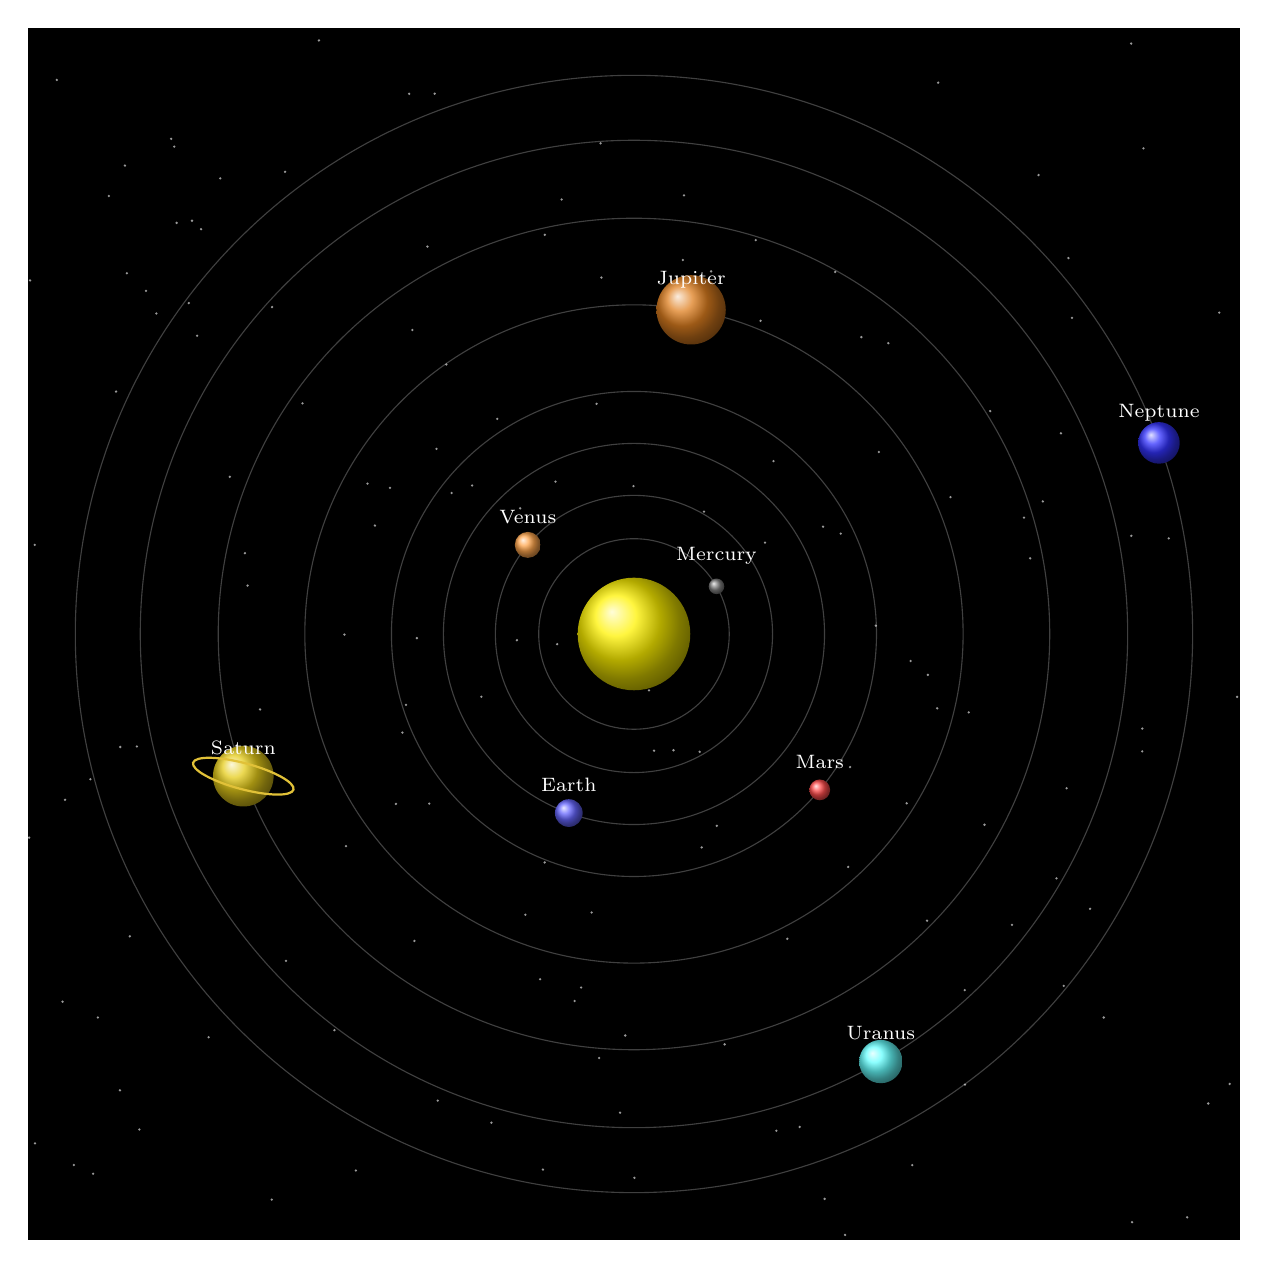
\begin{tikzpicture}[scale=0.55]
  \fill[black] (-14,-14) rectangle (14,14);
  \foreach \i in {1,...,160} {
    \pgfmathsetmacro\x{-14 + 28*rnd} \pgfmathsetmacro\y{-14 + 28*rnd}
    \fill[white, opacity=0.6] (\x,\y) circle (0.03);
  }
  \shade[ball color=yellow!90!orange] (0,0) circle (1.3);
  \foreach \r/\a/\s/\c/\name in {2.2/30/0.18/gray/Mercury, 3.2/140/0.3/orange!70/Venus, 4.4/250/0.32/blue!60/Earth,
      5.6/320/0.24/red!70/Mars, 7.6/80/0.8/orange!50!brown/Jupiter, 9.6/200/0.7/yellow!60!brown/Saturn,
      11.4/300/0.5/cyan!60/Uranus, 12.9/20/0.48/blue!80/Neptune} {
    \draw[white, opacity=0.25] (0,0) circle (\r);
    \shade[ball color=\c] (\a:\r) circle (\s);
    \node[white, font=\scriptsize, above=1.5mm] at (\a:\r) {\name};
  }
  \draw[yellow!50!brown, thick, rotate around={-15:(200:9.6)}] (200:9.6) ellipse (1.2 and 0.3);
\end{tikzpicture}
